\documentclass[11pt,a4paper]{article}
\usepackage[a4paper,margin=2.4cm]{geometry}
\usepackage{amsmath,amssymb,mathtools,amsthm}
\usepackage{fontspec}
\usepackage{polyglossia}
\setmainlanguage{russian}
\setotherlanguage{english}
\setmainfont{Liberation Serif}
\setsansfont{Liberation Sans}
\setmonofont{Liberation Mono}
\newfontfamily\cyrillicfont[Ligatures=TeX]{Liberation Serif}
\newfontfamily\cyrillicfontsf[Ligatures=TeX]{Liberation Sans}
\newfontfamily\cyrillicfonttt{Liberation Mono}
\usepackage{booktabs}
\usepackage{array}
\usepackage{enumitem}
\usepackage{graphicx}
\usepackage{float}
\usepackage{listings}
\usepackage{xcolor}
\usepackage[hidelinks]{hyperref}

\setlength{\parindent}{0pt}
\setlength{\parskip}{0.55em}
\emergencystretch=3em
\setlist{itemsep=0.25em,topsep=0.3em}
\lstset{basicstyle=\ttfamily\footnotesize,columns=fullflexible,keepspaces=true,
  frame=single,rulecolor=\color{black!25},breaklines=true,
  commentstyle=\color{black!55},showstringspaces=false,extendedchars=true}

\newcommand{\G}{\mathcal{G}_k}
\newcommand{\norm}[1]{\lVert #1\rVert_2}
\newcommand{\E}{\mathbb{E}}
\DeclareMathOperator*{\argmin}{arg\,min}
\DeclareMathOperator{\diag}{diag}
\DeclareMathOperator{\Var}{Var}
\renewcommand{\figurename}{Рис.}

\title{Раздел 2: реализация и численные проверки\\[0.2em]
\large на примере зашумлённой квадратичной функции}
\author{Homework Mini-Project: SGD versus Robust SGD under Gradient Uncertainty}
\date{17 ноября 2026 г.}

\begin{document}
\maketitle

\section*{Постановка и краткие результаты}

Раздел 2 требует четырёх вещей: (i) построить положительно определённую матрицу
неопределённости $S_k$ по наблюдениям градиентов отдельных примеров по формуле (4);
(ii) разработать численный метод для робастной подзадачи (2) и описать его критерий
остановки и вычислительную стоимость; (iii) реализовать SGD и R-SGD и получение
наблюдений градиента для обеих обучаемых моделей (пункт (a)); (iv) численно проверить
предел нулевого радиуса, изотропную формулу, правило нулевого шага и условие
оптимальности из 1(d) (пункт (b)), исследовать влияние размера батча (пункт (c)) и
описать всё необходимое для воспроизведения (пункт (d)). Все проверки выполнены на
зашумлённой квадратичной функции из раздела Illustration; оракулы градиентов обеих
обучаемых моделей также реализованы и проверены, чтобы раздел 3 использовал тот же код.

Основные результаты:
\begin{itemize}
\item \textbf{Решатель.} При диагональной $S_k$ задача (2) точно сводится к одному
скалярному уравнению относительно $\tau=\sqrt{d^TS_kd}$ — \emph{секулярному
уравнению}. Положительный корень существует тогда и только тогда, когда условие
нулевого шага (3) нарушено, поэтому решатель воспроизводит пункт 1(c) по построению.
Метод Ньютона для $\psi(\tau)=q(\tau)^{-1/2}-1$ сходится монотонно из $\tau_0=0$ (это
доказано: функция вогнута), в изотропном случае точен за одну итерацию, а на
20\,000 сильно анизотропных тестовых задачах потребовал в среднем 4.4 и не более 9
итераций. Стоимость одной итерации $O(p)$.
\item \textbf{Проверки.} Невязка условия 1(d) не превосходит $1.0\cdot10^{-14}$;
при $\rho=0$ SGD воспроизводится побитово; изотропная формула воспроизводится с
точностью $4.8\cdot10^{-12}$; правило нулевого шага совпадает с (3) в
$10\,000/10\,000$ случаев, включая $\rho=(1\pm10^{-6})\rho_c$.
\item \textbf{Размер батча.} $\widehat s_{k,j}$ — несмещённая оценка
$\Var(g_{k,j})=\Sigma_{jj}/b$, её относительный разброс равен $\sqrt{2/(b-1)}$ (141\%
при $b=2$, 9\% при $b=256$), а статистика $g^TS^{-1}g$ вдали от минимума растёт
линейно по $b$. Поэтому при фиксированном $\rho$ большой батч даёт меньшее сжатие
шага и меньше нулевых шагов; при $b\to\infty$ R-SGD переходит в SGD.
\end{itemize}

\begin{center}
\begin{tabular}{@{}llll@{}}
\toprule
Пункт задания & Что показано & Где & Итог \\
\midrule
$S_k$, формула (4) & несмещённость, роль $\varepsilon_k$ & шаг 1 & доказано, проверено \\
решатель для (2) & секулярное уравнение, Ньютон, стоимость & шаг 2 & доказано, замерено \\
(a) & SGD/R-SGD, наблюдения градиента & шаг 3 & ошибка КР $\le 5\cdot10^{-9}$ \\
(b) & четыре обязательных теста & шаг 4 & все пройдены \\
(c) & размер батча и $S_k$ & шаг 5 & теория = эксперимент \\
(d) & воспроизводимость & шаг 6 & сиды, настройки, версии \\
\bottomrule
\end{tabular}
\end{center}
(КР — конечные разности.)

\section*{Обозначения}

На итерации $k$ имеется $b\ge2$ наблюдений $v_{k,i}\in\mathbb R^p$ и
\begin{gather*}
g_k=\frac1b\sum_{i=1}^b v_{k,i},\qquad
\G=\{g_k+S_k^{1/2}u:\norm{u}\le\rho\},\\
d_k=\argmin_d\;\varphi_k(d),\qquad
\varphi_k(d)=g_k^Td+\rho\sqrt{d^TS_kd}+\frac{\norm{d}^2}{2\alpha_k}.
\end{gather*}
SGD делает шаг $\theta_{k+1}=\theta_k-\alpha_kg_k$, R-SGD — шаг
$\theta_{k+1}=\theta_k+d_k$. Внутри одного шага индекс $k$ опускается: $g$,
$S=\diag(s_1,\dots,s_p)$, $\alpha$. Норма Махаланобиса вектора $g$ и порог нулевого
шага:
\begin{equation*}
\kappa^2=g^TS^{-1}g=\sum_{j=1}^p\frac{g_j^2}{s_j},\qquad \rho_c=\kappa .
\end{equation*}

\textbf{Тестовая задача (Illustration).}
$f(\theta)=\tfrac12(\theta_1^2+4\theta_2^2)$, $\nabla f(\theta)=(\theta_1,4\theta_2)^T$,
гессиан $\diag(1,4)$, поэтому $L=4$ и $\mu=1$; $\theta_0=(2,2)^T$, $f(\theta_0)=10$,
$f^\star=0$. Наблюдения $v_{k,i}=\nabla f(\theta_k)+\sigma Az_{k,i}$, $A=\diag(2,\tfrac12)$,
$z_{k,i}\sim\mathcal N(0,I_2)$, так что ковариация одного наблюдения
\begin{equation*}
\Sigma=\sigma^2AA^T=\sigma^2\diag\big(4,\tfrac14\big).
\end{equation*}
Шум велик вдоль $\theta_1$, где кривизна мала, и мал вдоль $\theta_2$, где кривизна
велика: отношение сигнал/шум в двух направлениях сильно различается. Поскольку
$\Sigma$ диагональна, диагональная оценка (4) здесь ничего не теряет; в обучаемых
моделях она пренебрегает корреляциями между параметрами.

\section*{Шаг 1. Матрица неопределённости $S_k$ (формула (4))}

\begin{equation*}
\widehat s_{k,j}=\frac1{b(b-1)}\sum_{i=1}^b(v_{k,i,j}-g_{k,j})^2,\qquad
s_{k,j}=\widehat s_{k,j}+\varepsilon_k,\qquad
\varepsilon_k=10^{-3}\max\Big\{\frac1p\sum_j\widehat s_{k,j},\,10^{-8}\Big\}.
\end{equation*}

\subsection*{Что оценивает $\widehat s_{k,j}$}

Пусть при фиксированном $\theta_k$ наблюдения независимы и одинаково распределены со
средним $m$ и ковариацией $\Sigma$. Для обучаемых моделей именно это обеспечивает
выбор примеров \emph{с возвращением} (в шаге 5 показано, что происходит без него).
Тогда $\Var(g_{k,j})=\Sigma_{jj}/b$. Из тождества
\begin{equation*}
\sum_{i=1}^b(v_{i,j}-g_j)^2=\sum_{i=1}^b(v_{i,j}-m_j)^2-b\,(g_j-m_j)^2
\end{equation*}
после взятия математического ожидания получаем
$\E\sum_i(v_{i,j}-g_j)^2=b\Sigma_{jj}-\Sigma_{jj}=(b-1)\Sigma_{jj}$. Делим на $b(b-1)$:
\begin{equation*}
\boxed{\;\E\,\widehat s_{k,j}=\frac{\Sigma_{jj}}b=\Var(g_{k,j})\;}
\end{equation*}
Таким образом, $S_k$ — это (диагональ) ковариации \emph{среднего по батчу}, а не
одного наблюдения. Это правильный объект: множество $\G$ описывает неопределённость
именно $g_k$.

\subsection*{Положительная определённость и роль $\varepsilon_k$}

Каждое $s_{k,j}\ge\varepsilon_k\ge10^{-11}>0$, поэтому всегда $S_k\succ0$. Добавка
нужна в двух ситуациях: координата, по которой все наблюдения совпадают (например,
насыщенный нейрон $\tanh$ или смещение модели с одинаковыми градиентами примеров), и
квадратичная задача без шума ($\sigma=0$), где все $v_{k,i}$ совпадают и
$\widehat s_k=0$. Относительная часть $10^{-3}\cdot\text{mean}(\widehat s)$ делает
добавку инвариантной к масштабу: она ограничивает отношение $\max_js_j/\min_js_j$
величиной порядка $10^3p$. Абсолютная часть $10^{-11}$ работает, только когда все
$\widehat s_{k,j}$ равны нулю. Тогда $S_k=\varepsilon_kI$, и по изотропной формуле из 1(d)
шаг R-SGD равен $d_k=-\alpha_k(1-\rho\sqrt{\varepsilon_k}/\norm{g_k})_+g_k$. Это SGD с
относительным изменением $\rho\sqrt{\varepsilon_k}/\norm{g_k}$, кроме крошечной
области $\norm{g_k}\le\rho\sqrt{\varepsilon_k}\approx3.2\cdot10^{-6}\rho$; это
проверено численно в шаге 4.

\section*{Шаг 2. Решатель робастной подзадачи (2)}

\subsection*{2.1 Тривиальные случаи}
\begin{itemize}
\item $\rho=0$: $\varphi(d)=g^Td+\norm d^2/(2\alpha)$, откуда $d=-\alpha g$ (SGD),
пункт 1(b).
\item $\kappa^2=g^TS^{-1}g\le\rho^2$: $d=0$, пункт 1(c). Эта проверка точна и стоит
$O(p)$. Шаг считается \emph{нулевым} только тогда, когда сработала эта проверка, а не
по сравнению $\norm d$ с допуском. Случай $g=0$ сюда входит ($\kappa=0\le\rho$).
\end{itemize}

\subsection*{2.2 Сведение к одному скалярному уравнению}

Пусть $\rho>0$ и $\kappa>\rho$. По пункту 1(c) точка минимума $d\neq0$, поэтому
$\varphi$ в ней дифференцируема и выполнено условие из 1(d):
\begin{equation*}
g+\rho\frac{Sd}{\sqrt{d^TSd}}+\frac d\alpha=0 .
\end{equation*}
Введём неизвестный скаляр $\tau=\sqrt{d^TSd}>0$. Так как $S$ диагональна, векторное
уравнение распадается на $p$ скалярных: $g_j+\rho s_jd_j/\tau+d_j/\alpha=0$, то есть
$d_j\big(\tfrac1\alpha+\tfrac{\rho s_j}{\tau}\big)=-g_j$. Умножая на $\alpha\tau$,
получаем
\begin{equation*}
\boxed{\;d_j(\tau)=-\alpha\,\frac{\tau}{\tau+\alpha\rho s_j}\,g_j,\qquad j=1,\dots,p\;}
\end{equation*}
При любом $\tau>0$ вектор $d(\tau)$ удовлетворяет условию оптимальности, \emph{в
котором $\sqrt{d^TSd}$ заменено на $\tau$}. Решением он является тогда и только тогда,
когда $\tau$ согласовано со своим определением: $\tau^2=\sum_js_jd_j(\tau)^2$.
Подставляя $d_j(\tau)$ и деля на $\tau^2>0$, получаем \emph{секулярное уравнение}
\begin{equation*}
q(\tau):=\sum_{j=1}^p\frac{a_j}{(\tau+c_j)^2}=1,\qquad
a_j=\alpha^2s_jg_j^2\ge0,\quad c_j=\alpha\rho s_j>0 .
\end{equation*}
(Название пришло из подзадачи доверительной области, где возникает уравнение того же
вида; см.\ Moré, Sorensen, 1983; Nocedal, Wright, 2006, §4.3.)

\subsection*{2.3 Существование и единственность корня $\Longleftrightarrow$ (3) нарушено}

Так как $g\ne0$, хотя бы одно $a_j>0$, и
\begin{equation*}
q'(\tau)=-2\sum_j\frac{a_j}{(\tau+c_j)^3}<0\quad(\tau\ge0),\qquad
q(0)=\sum_j\frac{\alpha^2s_jg_j^2}{\alpha^2\rho^2s_j^2}=\frac{\kappa^2}{\rho^2},\qquad
\lim_{\tau\to\infty}q(\tau)=0 .
\end{equation*}
Функция $q$ непрерывна и строго убывает, поэтому уравнение $q(\tau)=1$ имеет корень на
$(0,\infty)$ тогда и только тогда, когда $q(0)>1$, то есть $\kappa>\rho$, и этот корень
$\tau^\star$ единственен. При $\kappa\le\rho$ корня нет, то есть ни одна ненулевая
точка не удовлетворяет условию оптимальности, и минимум (он существует, поскольку
$\varphi$ сильно выпукла) обязан достигаться в $d=0$. Тем самым правило нулевого шага
1(c) содержится в решателе как случай отсутствия корня его собственного уравнения.
Поскольку задача (2) $1/\alpha$-сильно выпукла, стационарная точка $d(\tau^\star)$ —
её единственный глобальный минимум.

\textbf{Отрезок локализации.} Так как $c_j>0$, имеем
$q(\tau)\le\sum_ja_j/\tau^2=\alpha^2g^TSg/\tau^2$. Значит, $q(\tau_{\rm hi})\le1$ при
$\tau_{\rm hi}=\alpha\sqrt{g^TSg}$, и $\tau^\star\in(0,\tau_{\rm hi}]$.

\subsection*{2.4 Метод Ньютона для $\psi(\tau)=q(\tau)^{-1/2}-1$}

Вместо $q(\tau)-1$ (выпуклой функции, ведущей себя как $1/\tau^2$) решается уравнение
$\psi(\tau)=q(\tau)^{-1/2}-1=0$. Функция $\psi$ возрастает ($q$ убывает) и обладает
следующим ключевым свойством.

\textbf{Лемма (вогнутость).} $\psi$ вогнута на $[0,\infty)$; она аффинна тогда и
только тогда, когда все $s_j$ с $g_j\ne0$ равны между собой.

\emph{Доказательство.} Обозначим $x_j=1/(\tau+c_j)$ и $A_m=\sum_ja_jx_j^m$. Тогда
$q=A_2$, $q'=-2A_3$, $q''=6A_4$. Для $F=q^{-1/2}$
\begin{equation*}
F'=-\tfrac12q^{-3/2}q',\qquad
F''=q^{-5/2}\Big(\tfrac34q'^2-\tfrac12q\,q''\Big)=3\,q^{-5/2}\big(A_3^2-A_2A_4\big).
\end{equation*}
По неравенству Коши — Буняковского для векторов $(\sqrt{a_j}\,x_j)_j$ и
$(\sqrt{a_j}\,x_j^2)_j$ имеем $A_3^2\le A_2A_4$, поэтому $F''\le0$. Равенство
достигается тогда и только тогда, когда эти векторы пропорциональны, то есть $x_j$
одинаковы для всех $j$ с $a_j>0$, то есть все такие $c_j=\alpha\rho s_j$ совпадают.
\hfill$\blacksquare$

\textbf{Монотонная сходимость из $\tau_0=0$.} Имеем $\psi(0)=\rho/\kappa-1<0$.
Итерация Ньютона: $\tau_{n+1}=\tau_n-\psi(\tau_n)/\psi'(\tau_n)$, где $\psi'>0$. В силу
вогнутости касательная лежит не ниже графика:
$\psi(\tau)\le\psi(\tau_n)+\psi'(\tau_n)(\tau-\tau_n)$. В точке $\tau=\tau_{n+1}$
правая часть равна нулю, поэтому $\psi(\tau_{n+1})\le0$, то есть
$\tau_{n+1}\le\tau^\star$. Кроме того,
$\tau_{n+1}-\tau_n=-\psi(\tau_n)/\psi'(\tau_n)\ge0$. Итерации монотонно возрастают и
остаются не выше $\tau^\star$; их предел $\bar\tau$ удовлетворяет $\psi(\bar\tau)=0$
(непрерывность и $\psi'\ge\psi'(\tau^\star)>0$ на $[0,\tau^\star]$ в силу вогнутости),
поэтому $\bar\tau=\tau^\star$. Так как $\psi$ гладкая и $\psi'(\tau^\star)>0$,
сходимость локально квадратичная. В изотропном случае $\psi$ аффинна, и первый же шаг
Ньютона попадает точно в $\tau^\star$.

Почему $q^{-1/2}$, а не $q-1$: в изотропном случае $q^{-1/2}=(\tau+c)/\sqrt{\sum a_j}$ —
прямая, а при анизотропии функция остаётся близкой к прямой, поэтому Ньютону нужно
очень мало шагов. Для $q-1$ метод Ньютона из $\tau_0=0$ тоже монотонен (выпуклая
убывающая функция), но сходится гораздо медленнее.

\textbf{Страховка.} Итерация хранит отрезок $[\tau_{\rm lo},\tau_{\rm hi}]$ и заменяет
любую итерацию Ньютона, вышедшую за него, шагом бисекции. По доказанному выше в точной
арифметике этого не происходит; на 20\,000 тестовых задачах страховка не сработала ни
разу.

\subsection*{2.5 Критерий остановки и апостериорная проверка}

Итерации прекращаются, когда $|\psi(\tau_n)|\le10^{-14}$, или когда изменение
$|\tau_{n+1}-\tau_n|\le10^{-15}\tau_{n+1}$, или после 100 итераций (наблюдаемый
максимум — 9). Возвращается $d=d(\tau_n)$.

Что контролирует критерий: $d(\tau)$ удовлетворяет условию оптимальности точно, с
$\tau$ вместо $\sqrt{d^TSd}$, и
$\sqrt{d(\tau)^TSd(\tau)}=\tau\sqrt{q(\tau)}=\tau/(1+\psi(\tau))$. Значит, единственная
ошибка — относительное расхождение $|\psi|$ между $\tau$ и $\sqrt{d^TSd}$. После решения
код дополнительно вычисляет невязку условия 1(d)
\begin{equation*}
r(d)=\frac{\norm{g+\rho Sd/\sqrt{d^TSd}+d/\alpha}}{\norm g}
\end{equation*}
и сохраняет её (шаг 4).

\subsection*{2.6 Вычислительная стоимость}

\begin{itemize}
\item Предвычисление $a_j$, $c_j$, $\kappa^2$ стоит $O(p)$; каждая итерация Ньютона
вычисляет две суммы, $O(p)$; память $O(p)$. Итого $O(p\cdot n_{\rm it})$, где
наблюдалось $n_{\rm it}\le9$.
\item Построение $g_k$ и $S_k$ по $V\in\mathbb R^{b\times p}$ стоит $O(bp)$, а
вычисление $b$ градиентов отдельных примеров — $O(b\cdot\text{(один backprop)})$, что
уже не меньше $O(bp)$. Асимптотически решатель дешевле данных, которые он получает,
примерно в $b/n_{\rm it}$ раз.
\item \textbf{Измеренное время (Python/NumPy, одно ядро).} Решатель: 37\,мкс при
$p=3$, 43\,мкс при $p=33$, 82\,мкс при $p=1000$, 4.7\,мс при $p=10^5$ (линейный рост
при больших $p$). Для сравнения, для сети с 33 параметрами и $b=32$: градиенты примеров
18\,мкс, построение $S_k$ 11\,мкс. Для таких маленьких моделей время решателя
определяется накладными расходами Python и \emph{не} пренебрежимо: одно обновление
R-SGD по времени стоит примерно в 2--4 раза больше обновления SGD, хотя оба используют
ровно $b$ вычислений градиента. Это нужно указать в разделе 3 (время работы — обязательный
результат).
\item Общая (недиагональная) $S\succ0$ сводится к диагональному случаю одним
спектральным разложением $S=Q\Lambda Q^T$ за $O(p^3)$: при $\tilde d=Q^Td$,
$\tilde g=Q^Tg$ задача принимает вид
$\tilde g^T\tilde d+\rho\sqrt{\tilde d^T\Lambda\tilde d}+\norm{\tilde d}^2/(2\alpha)$,
так как $Q$ сохраняет евклидову норму, и применяется тот же решатель.
\end{itemize}

\subsection*{2.7 Что формула говорит о робастном шаге}

Формула $d_j=-\alpha\,\frac{\tau^\star}{\tau^\star+\alpha\rho s_j}\,g_j$ показывает, что
R-SGD — это SGD со \emph{своим коэффициентом сжатия из $(0,1)$ для каждой
координаты}: чем неопределённее координата (чем больше $s_j$), тем сильнее она сжимается.
Поучительны два предела.
\begin{itemize}
\item $\rho\to0$: $\tau^\star\to\alpha\sqrt{g^TSg}$, все коэффициенты стремятся к 1,
$d\to-\alpha g$.
\item $\rho\uparrow\rho_c=\kappa$: $q(0)=\kappa^2/\rho^2\downarrow1$, поэтому
$\tau^\star\to0$. Тогда $\tau^\star\ll\alpha\rho s_j$ и
$d_j\approx-\tau^\star g_j/(\rho s_j)$: шаг обращается в ноль \emph{непрерывно}, а его
\emph{направление} стремится к $-S^{-1}g$, то есть к градиенту, измеренному в единицах
его собственной неопределённости.
\end{itemize}
Итак, при анизотропной $S$ рост $\rho$ поворачивает шаг от направления SGD $-g$ к
$-S^{-1}g$ и одновременно укорачивает его; при изотропной $S$ направление остаётся $-g$
и меняется только длина. Оба эффекта видны на рис.~\ref{fig:sweep}.

\section*{Шаг 3. Пункт (a): реализация SGD и R-SGD}

\subsection*{3.1 Одна итерация}

Оба метода выполняются одним циклом; различается только шаг.
\begin{enumerate}
\item Получить наблюдения $V\in\mathbb R^{b\times p}$, $V_{i\cdot}=v_{k,i}^T$ (п.~3.2).
\item $g_k$ — среднее строк $V$; $\widehat s_k$, $\varepsilon_k$, $s_k$ — по (4).
\item $\alpha_k=\alpha_0/\sqrt{1+k/50}$ (одно и то же расписание для обоих методов).
\item SGD: $d_k=-\alpha_kg_k$. R-SGD: $d_k=$ \texttt{robust\_step}$(g_k,s_k,\alpha_k,\rho)$
(шаг 2); при этом записывается, был ли шаг нулевым, а также $\kappa_k^2$, число итераций
Ньютона и невязка $r(d_k)$.
\item $\theta_{k+1}=\theta_k+d_k$.
\end{enumerate}
SGD нужен только $g_k$, но он получает ту же матрицу $V$, поэтому оба метода используют
ровно $b$ вычислений градиента на обновление, то есть $bK$ за запуск. Матрица $S_k$
строится по \emph{тем же} наблюдениям $V$, из которых получен $g_k$, как требует раздел 3
(«construct the uncertainty model from the gradient observations actually used in the
update»).

\subsection*{3.2 Откуда берутся наблюдения градиента}

Все три оракула имеют один интерфейс \texttt{observe(theta, rng\_batch, rng\_noise)}
$\to V$.

\textbf{Зашумлённая квадратичная функция.} $V=\mathbf 1\,\nabla f(\theta_k)^T+\sigma ZA^T$,
где $Z\in\mathbb R^{b\times2}$ — стандартная нормальная матрица; набора данных нет.

\textbf{Обучаемые модели.} Индексы $i_1,\dots,i_b$ выбираются независимо и равномерно из
$\{1,\dots,n\}$ \emph{с возвращением}; чистые градиенты отдельных примеров
$u_{i}(\theta_k)=\nabla_\theta\ell(t_\theta(a_{i}),y_{i})$ вычисляются по явным формулам
сразу для всего батча, и искажение добавляется только к ним:
$v_{k,i}=u_{i}(\theta_k)+\sigma z_{k,i}$, $z_{k,i}\sim\mathcal N(0,I_p)$. Обучающие
данные, целевая функция и все вычисления потерь и точности остаются чистыми.

\emph{Почему нужны градиенты отдельных примеров, а не градиент потерь на батче:}
$S_k$ строится по разбросу отдельных $v_{k,i}$ вокруг $g_k$, поэтому все $b$ векторов
нужны по отдельности. В фреймворке автоматического дифференцирования для этого
используют, например, \texttt{torch.func.vmap(grad(...))}; здесь явные формулы ниже
дешевле и точны.

\textbf{Логистическая регрессия} ($t=w^Ta+c$, $\theta=(w_1,w_2,c)$, $p=3$). Для
$\ell(t,y)=\log(1+e^t)-yt$
\begin{equation*}
\frac{\partial\ell}{\partial t}=\frac{e^t}{1+e^t}-y=\operatorname{sigm}(t)-y,\qquad
\nabla_\theta t=(a^T,1)^T\quad\Longrightarrow\quad
u_i(\theta)=\big(\operatorname{sigm}(t_i)-y_i\big)\begin{pmatrix}a_i\\1\end{pmatrix}.
\end{equation*}
Потери вычисляются устойчиво как \texttt{logaddexp(0,t)~-~y*t}, а сигмоида —
функцией \texttt{scipy.special.expit}.

\textbf{Двухслойная сеть} ($t=w_2^T\tanh(W_1a+b_1)+b_2$, $p=16+8+8+1=33$, порядок
параметров $(\mathrm{vec}_{\rm row}W_1,b_1,w_2,b_2)$). При $z=W_1a+b_1$, $h=\tanh z$,
$\delta=\operatorname{sigm}(t)-y$ обратное распространение даёт
\begin{equation*}
\frac{\partial\ell}{\partial b_2}=\delta,\quad
\frac{\partial\ell}{\partial w_2}=\delta\,h,\quad
\frac{\partial\ell}{\partial b_1}=\delta\,w_2\odot(1-h\odot h)=:e,\quad
\frac{\partial\ell}{\partial W_1}=e\,a^T,
\end{equation*}
что вычисляется для всех $b$ примеров через broadcasting (матрица $b\times33$).
Документированная инициализация (для раздела 3): $W_1\sim\mathcal N(0,\tfrac12)$,
$b_1=0$, $w_2\sim\mathcal N(0,\tfrac18)$, $b_2=0$ (дисперсия $1/\text{fan-in}$).

\textbf{Проверка конечными разностями.} Для 5 случайных векторов параметров на модель
(200 точек каждого набора данных) центральные разности с $h=10^{-6}$ сравнивались (i)
для среднего градиентов примеров с градиентом средних потерь и (ii) для каждого из 20
градиентов примеров с потерями на одном примере:

\begin{center}
\begin{tabular}{@{}lcc@{}}
\toprule
Модель & \shortstack{макс.\ отн.\ ошибка,\\ средний градиент} & \shortstack{макс.\ отн.\ ошибка,\\ по примерам} \\
\midrule
логистическая регрессия ($p=3$) & $3.2\cdot10^{-10}$ & $4.6\cdot10^{-9}$ \\
двухслойная сеть ($p=33$) & $6.3\cdot10^{-10}$ & $5.3\cdot10^{-10}$ \\
\bottomrule
\end{tabular}
\end{center}
Эти ошибки находятся на уровне погрешности самих конечных разностей (усечение
$\approx h^2$ и округление $\approx\epsilon_{\rm mach}/h$), поэтому аналитические
градиенты верны.

\section*{Шаг 4. Пункт (b): численные проверки}

Случайные тестовые задачи для решателя намеренно трудные: $g\sim\mathcal N(0,I_p)$,
$s_j$ логравномерно на шести порядках $[10^{-3},10^3]$, $\alpha$ логравномерно на
$[10^{-2},1]$, $p\in\{2,3,33,1000\}$, $\rho=m\rho_c$ с $m$, выбираемым как указано
ниже. Все числа этого отчёта получены скриптом \texttt{checks\_section2.py} и
сохранены в \texttt{results\_section2.json}.

\subsection*{4.1 Предел нулевого радиуса}
\begin{itemize}
\item Ровно $\rho=0$: $d=-\alpha g$ побитово в $1000/1000$ случайных задач ($p$ от 1
до 49).
\item $\rho\to0^+$: для пяти задач с $p=33$ и $\rho=10^{-1},\dots,10^{-8}$ отклонение
$\norm{d(\rho)+\alpha g}/(\alpha\norm g)$ убывает линейно по $\rho$; наклоны в
двойном логарифмическом масштабе $0.995$--$0.999$, при $\rho=10^{-8}$ отклонение не
больше $1.5\cdot10^{-8}$. Робастный шаг непрерывен в $\rho=0$, изменение первого
порядка.
\item Траектории: SGD и R-SGD с $\rho=0$ на квадратичной задаче ($\sigma=1$, $b=8$,
300 обновлений) с одинаковыми сидами совпадают точно (максимальная разность 0).
\end{itemize}

\subsection*{4.2 Изотропная формула}

$10\,000$ задач с $S=sI$: $p\in\{1,\dots,50\}$, $s$ логравномерно на
$[10^{-4},10^2]$, $\rho$ выбрано так, что отношение $\rho\sqrt s/\norm g$ равномерно на
$[0,2]$ — это одинаково покрывает обе ветви $(\cdot)_+$. Решатель сравнивался с
\begin{equation*}
d=-\alpha\Big(1-\frac{\rho\sqrt s}{\norm g}\Big)_+g .
\end{equation*}
\begin{itemize}
\item ветвь (нулевой или ненулевой шаг) совпала в $10\,000/10\,000$ случаев (4949
нулевых шагов);
\item для 5051 ненулевого шага максимальная относительная ошибка $4.8\cdot10^{-12}$;
\item каждый ненулевой шаг занял ровно \textbf{одну} итерацию Ньютона, как и
предсказывает лемма из 2.4 ($\psi$ аффинна);
\item $g=0$ даёт $d=0$ через проверку нулевого шага, как требует 1(d).
\end{itemize}

\subsection*{4.3 Правило нулевого шага}

Для каждого $m\in\{0.5,0.9,0.99,0.999,1-10^{-6},1+10^{-6},1.001,1.01,1.1,2\}$ решено
1000 анизотропных задач с $\rho=m\rho_c$. Решатель вернул ровно $d=0$ тогда и только
тогда, когда $m>1$, — в $1000/1000$ случаев для каждого $m$, включая $m=1\pm10^{-6}$.
Рис.~\ref{fig:sweep}(a) показывает, что $\norm d$ непрерывно стремится к нулю при
$\rho\uparrow\rho_c$ и остаётся нулём дальше; панель (b) показывает поворот
направления от $-g$ к $-S^{-1}g$, предсказанный в 2.7 (в этом примере угол между $g$ и
$S^{-1}g$ равен $57.8^\circ$).

\begin{figure}[H]
\centering
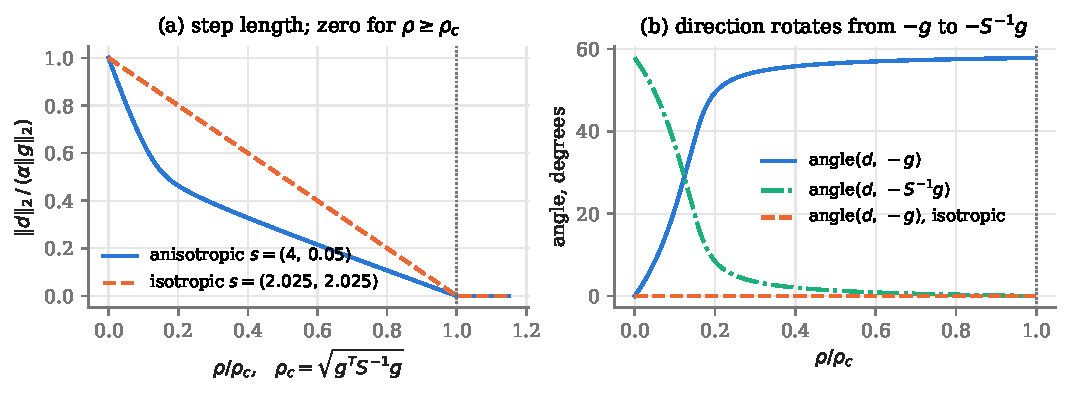
\includegraphics[width=\linewidth]{../fig/zero_step_sweep.pdf}
\caption{Робастный шаг для $g=(1,\,0.6)$, $\alpha=0.5$ как функция $\rho/\rho_c$.
Анизотропная $s=(4,\,0.05)$, $\rho_c=2.73$; изотропная $s$ с тем же средним,
$\rho_c=0.82$. (a) Длина шага относительно SGD; ровно при $\rho=\rho_c$ она становится
нулевой. (b) Угол между $d$ и $-g$ и между $d$ и $-S^{-1}g$; при изотропной $S$
направление не меняется. (Подписи на рисунке на английском.)}
\label{fig:sweep}
\end{figure}

\subsection*{4.4 Условие оптимальности из 1(d) и независимые проверки}

\begin{center}
\begin{tabular}{@{}p{0.47\linewidth}p{0.45\linewidth}@{}}
\toprule
Проверка & Результат \\
\midrule
Невязка $r(d)$ из 1(d), 20\,000 случайных задач, $m\sim U(0.001,0.999)$ &
$\max r=1.0\cdot10^{-14}$ \\
Невязка на всех траекториях R-SGD из 4.5 & $\max r=9.9\cdot10^{-15}$ \\
Итерации Ньютона, 20\,000 задач &
среднее 4.4, медиана 4, квантиль 99\% — 7, максимум 9 \\
Шаги бисекции / немонотонные итерации Ньютона & $0$ / $0$ (5000 запусков без страховки) \\
Седловая точка (1): $d=-\alpha h^\star$, $h^\star=g+\rho Sd/\sqrt{d^TSd}$ (пункт 1(a)) &
$\max\norm{d+\alpha h^\star}/\norm d=6.0\cdot10^{-12}$ \\
CVXPY (Clarabel), форма SOCP, 300 задач ($s_j$ на четырёх порядках, $m\sim U(0.05,0.95)$) &
наша целевая функция ни разу не больше: $\max(\varphi_{\rm наш}-\varphi_{\rm cvx})/|\varphi|=1.8\cdot10^{-15}$ \\
& $\norm{d-d_{\rm cvx}}/\norm d$: медиана $4.0\cdot10^{-7}$, максимум $4.0\cdot10^{-4}$ \\
Сертификат сильной выпуклости
$\varphi(d+\delta)-\varphi(d)\ge\norm\delta^2/(2\alpha)$, 15\,000 случайных $\delta$ &
наименьший относительный запас $-1.6\cdot10^{-15}$ (только округление) \\
\bottomrule
\end{tabular}
\end{center}

Замечания.
\begin{itemize}
\item Форма SOCP для CVXPY:
$\min_{d,t}\;g^Td+\rho t+\norm d^2/(2\alpha)$ при $\norm{S^{1/2}d}\le t$. Её решения
отличаются от наших до $4\cdot10^{-4}$, потому что метод внутренней точки достигает
точности по целевой функции лишь около $10^{-8}$ (Clarabel пометил 135 из 300 решений как
«optimal\_inaccurate» при запрошенном допуске $10^{-12}$). Так как $\varphi$
$1/\alpha$-сильно выпукла,
$\norm{d_{\rm cvx}-d^\star}^2\le2\alpha(\varphi(d_{\rm cvx})-\varphi(d^\star))$, и разрыв
$10^{-8}$ по целевой функции объясняет расстояние $10^{-4}$. Наша целевая функция ни
разу не оказалась больше, чем у CVXPY.
\item Тест сертификата — прямое доказательство оптимальности: для точного минимума
$1/\alpha$-сильно выпуклой функции неравенство выполнено при любом $\delta$, а в
неоптимальной точке оно нарушается для малых $\delta$ вдоль направления убывания.
\item Ошибка седловой точки — это та же невязка, измеренная иначе:
$d+\alpha h^\star=\alpha\,(g+\rho Sd/\tau+d/\alpha)$, поэтому она умножена на
$\alpha\norm g/\norm d$, что велико чуть ниже порога.
\end{itemize}

\subsection*{4.5 Нулевые шаги на траекториях зашумлённой квадратичной задачи}

Это иллюстрация, а не настроенное сравнение: $b=8$, $\alpha_0=0.2$ (меньше
$2/L=0.5$), $\alpha_k=\alpha_0/\sqrt{1+k/50}$, $K=300$ обновлений, $\theta_0=(2,2)$,
20 сидов с общими случайными числами (оба метода получают одни и те же $z_{k,i}$),
$\rho\in\{1,\,2.45\}$. Значение $2.45\approx\sqrt{\chi^2_{2,0.95}}$ — радиус, при
котором при большом $b$ 95\% обновлений в точке минимума оказываются нулевыми (шаг 5).

\begin{center}
\small
\begin{tabular}{@{}llcccc@{}}
\toprule
$\sigma$ & метод & \shortstack{медиана итогового\\ $f$ [IQR]} & \shortstack{нулевые\\ шаги} & \shortstack{макс.\ $f$ при\\ нулевом шаге} & \shortstack{ср.\ итераций\\ Ньютона} \\
\midrule
0 & SGD & $6.3\cdot10^{-31}$ & -- & -- & -- \\
0 & R-SGD $\rho=1$ & $5.0\cdot10^{-12}$ & 0 & -- & 1.0 \\
0 & R-SGD $\rho=2.45$ & $3.0\cdot10^{-11}$ & 0 & -- & 1.0 \\
\midrule
1 & SGD & $0.0034$ [0.0020, 0.0067] & -- & -- & -- \\
1 & R-SGD $\rho=1$ & $0.0016$ [0.0005, 0.0073] & 33.0\% & 0.94 & 4.3 \\
1 & R-SGD $\rho=2.45$ & $0.0196$ [0.0085, 0.0386] & 80.8\% & 1.59 & 4.1 \\
\midrule
4 & SGD & $0.054$ [0.033, 0.107] & -- & -- & -- \\
4 & R-SGD $\rho=1$ & $0.026$ [0.008, 0.116] & 33.7\% & 2.50 & 4.3 \\
4 & R-SGD $\rho=2.45$ & $0.126$ [0.027, 0.269] & 85.0\% & 2.94 & 3.9 \\
\bottomrule
\end{tabular}
\end{center}
(IQR — интерквартильный размах по 20 сидам.)

\begin{figure}[H]
\centering
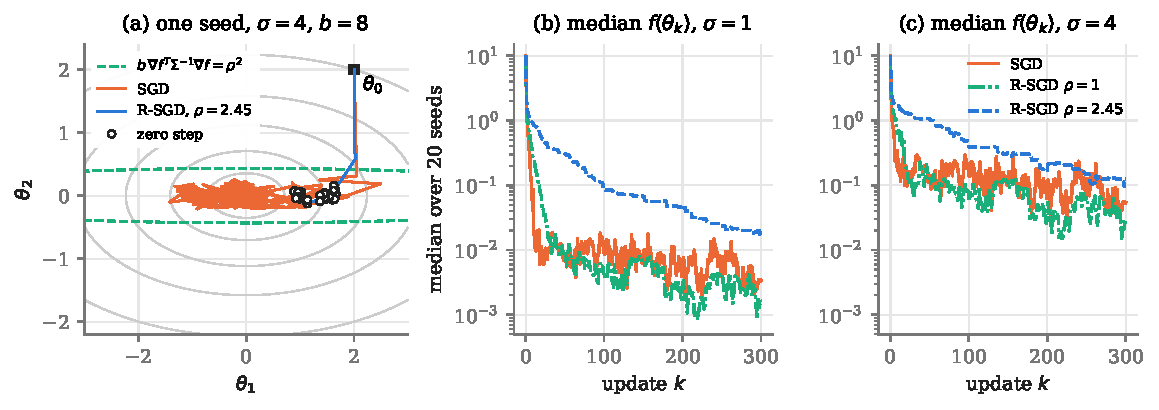
\includegraphics[width=\linewidth]{../fig/quadratic_trajectories.pdf}
\caption{Зашумлённая квадратичная задача, $b=8$, $\alpha_0=0.2$, 300 обновлений.
(a) Один сид при $\sigma=4$: SGD и R-SGD ($\rho=2.45$) с одинаковыми реализациями шума;
кружки отмечают точки, где R-SGD сделал нулевой шаг; пунктирный эллипс —
$b\,\nabla f^T\Sigma^{-1}\nabla f=\rho^2$ (полуоси $6.9$ и $0.43$, поэтому в этом окне он
выглядит как горизонтальная полоса). (b), (c) Медиана $f(\theta_k)$ по 20 сидам.}
\label{fig:traj}
\end{figure}

Что показывают эти числа:
\begin{itemize}
\item \textbf{Нулевые шаги происходят далеко от минимума.} При $\sigma=4$,
$\rho=2.45$ нулевые шаги случались в точках с $f$ до $2.94$ (при $f(\theta_0)=10$ и
$f^\star=0$), где $\norm{\nabla f}$ далеко не ноль. Рис.~\ref{fig:traj}(a) объясняет
почему: вдоль $\theta_1$ градиент $\theta_1$ слабый, а шум сильный (стандартное
отклонение $2\sigma$ на наблюдение), поэтому ожидаемая статистика
$b\,\nabla f^T\Sigma^{-1}\nabla f=b\big(\theta_1^2/(4\sigma^2)+64\theta_2^2/\sigma^2\big)$
остаётся меньше $\rho^2$ при $|\theta_1|$ вплоть до $\rho\cdot2\sigma/\sqrt b=6.9$.
R-SGD быстро исправляет $\theta_2$, где отношение сигнал/шум велико, а затем
останавливается по $\theta_1$. Это численное подтверждение ответа на 1(c): из (3) не
следует $\nabla f(\theta_k)=0$.
\item \textbf{Добавка $\varepsilon_k$ при $\sigma=0$.} Все наблюдения совпадают,
$S_k=10^{-11}I$, и R-SGD сходится к границе своей области нулевого шага
$\norm{\nabla f}=\rho\sqrt{\varepsilon}$, где
$f\approx\norm{\nabla f}^2/2=\rho^2\varepsilon/2$: $5.0000\cdot10^{-12}$ при $\rho=1$
и $3.0013\cdot10^{-11}$ при $\rho=2.45$, что совпадает с измеренными медианами до
девяти знаков. Приближение к границе непрерывно, поэтому ни одного точного нулевого шага
не зафиксировано. Так как $S=\varepsilon I$ изотропна, Ньютон на каждом обновлении
делал одну итерацию.
\item \textbf{Умеренный радиус может помочь, большой — тормозит.} $\rho=1$ уменьшил
медиану итогового $f$ (0.0016 против 0.0034 при $\sigma=1$; 0.026 против 0.054 при
$\sigma=4$), но интерквартильные размахи перекрываются, а $\rho=2.45$ оказался хуже SGD
при обоих уровнях шума. Это ненастроенные иллюстративные запуски; сохранится ли выигрыш
при честной настройке $\alpha_0$ для обоих методов и сводится ли он к укорочению шага —
вопрос разделов 4--5.
\item \textbf{Стоимость.} Оба метода потратили $2400=bK$ вычислений градиента за
запуск; время — около 4--7\,мс на запуск для SGD и 9--23\,мс для R-SGD (запуски с
большим числом нулевых шагов быстрее, так как нулевой шаг не вызывает Ньютона).
\end{itemize}

\section*{Шаг 5. Пункт (c): как размер батча влияет на оценку неопределённости}

\subsection*{5.1 Теория}

Зафиксируем $\theta$ и будем считать наблюдения гауссовскими, как в квадратичной задаче:
$v_{i,j}\sim\mathcal N(\mu_j,\Sigma_{jj})$ независимо, с независимыми координатами
($A$ диагональна). Из стандартных фактов о гауссовских выборках следует:
\begin{enumerate}
\item \textbf{Среднее.} $\E\widehat s_j=\Sigma_{jj}/b$ (шаг 1): сама оценка убывает как
$1/b$, потому что она оценивает дисперсию среднего.
\item \textbf{Разброс.} $(b-1)\,b\,\widehat s_j/\Sigma_{jj}\sim\chi^2_{b-1}$, отсюда
$\operatorname{sd}(\widehat s_j)/\E\widehat s_j=\sqrt{2/(b-1)}$: 141\% при $b=2$, 53\%
при $b=8$, 9\% при $b=256$. При маленьком батче сама $S_k$ очень шумная.
\item \textbf{Статистика нулевого шага.} $g_j$ и $\widehat s_j$ независимы, и
$\E[1/\chi^2_\nu]=1/(\nu-2)$, поэтому (без учёта $\varepsilon_k$)
\begin{align*}
\E\big[g^TS^{-1}g\big]&=\sum_j\E[g_j^2]\,\E[1/\widehat s_j]
=\sum_j\Big(\mu_j^2+\frac{\Sigma_{jj}}b\Big)\frac{b}{\Sigma_{jj}}\,\frac{b-1}{b-3}\\
&=\big(b\,\mu^T\Sigma^{-1}\mu+p\big)\frac{b-1}{b-3},\qquad b>3 .
\end{align*}
Вдали от стационарной точки ($\mu\ne0$) статистика растёт \emph{линейно} по $b$,
поэтому при фиксированном $\rho$ нулевые шаги с ростом $b$ исчезают. В стационарной
точке ($\mu=0$) каждое $g_j/\sqrt{\widehat s_j}$ имеет распределение Стьюдента с $b-1$
степенями свободы, среднее равно $p(b-1)/(b-3)$, а при $b\le3$ оно бесконечно (тяжёлые
хвосты). При больших $b$ $g^TS^{-1}g\to\chi^2_p$ по распределению, что задаёт
естественный масштаб для $\rho$: $\rho=\sqrt{\chi^2_{p,0.95}}$ ($=2.45$ при $p=2$)
означает 95\% нулевых шагов в точке минимума.
\item \textbf{Величина робастной поправки.} Радиус неопределённости в единицах
градиента $\rho\sqrt{s_j}\propto\rho/\sqrt b$, поэтому коэффициенты сжатия из 2.7
стремятся к 1, и при фиксированном $\rho$ и $b\to\infty$ R-SGD переходит в SGD. Иначе
говоря, $\rho$ и $b$ — не независимые параметры: один и тот же $\rho$ означает разную
степень робастности при разных размерах батча.
\end{enumerate}

\subsection*{5.2 Численная проверка}

$\sigma=1$ (так что $\Sigma=\diag(4,\tfrac14)$), $20\,000$ независимых батчей для
каждого $b$, в трёх фиксированных точках: минимум $\theta^\star=(0,0)$, промежуточная
точка $\theta_{\rm mid}=(1,\,0.1)$ с $\mu^T\Sigma^{-1}\mu=0.89$ и $\theta_0=(2,2)$ с
$\mu^T\Sigma^{-1}\mu=257$. Нулевые шаги считаются при $\rho=2.45$; последний столбец —
среднее относительное изменение шага $\norm{d+\alpha g}/(\alpha\norm g)$ в
$\theta_{\rm mid}$ при $\rho=1$, $\alpha=0.1$.

\begin{center}
\small
\setlength{\tabcolsep}{4.0pt}
\begin{tabular}{@{}rccccccccc@{}}
\toprule
& \multicolumn{2}{c}{$b\,\E\widehat s_j/\Sigma_{jj}$} & \multicolumn{2}{c}{отн.\ разброс $\widehat s_1$}
& \multicolumn{2}{c}{$\E\,g^TS^{-1}g$ в $\theta^\star$} & \multicolumn{2}{c}{доля нулевых шагов} & отн.\ изм. \\
\cmidrule(lr){2-3}\cmidrule(lr){4-5}\cmidrule(lr){6-7}\cmidrule(lr){8-9}
$b$ & $j=1$ & $j=2$ & эмп. & $\sqrt{2/(b-1)}$ & эмп. & теория & $\theta^\star$ & $\theta_{\rm mid}$ & в $\theta_{\rm mid}$ \\
\midrule
2 & 1.002 & 1.013 & 1.415 & 1.414 & 788.47 & $\infty$ & 0.558 & 0.410 & 0.579 \\
3 & 0.998 & 1.011 & 1.011 & 1.000 & 13.27 & $\infty$ & 0.719 & 0.484 & 0.606 \\
4 & 1.003 & 1.000 & 0.819 & 0.816 & 5.32 & 6.00 & 0.794 & 0.479 & 0.604 \\
8 & 0.994 & 0.999 & 0.534 & 0.535 & 2.78 & 2.80 & 0.885 & 0.297 & 0.536 \\
16 & 0.999 & 1.003 & 0.365 & 0.365 & 2.30 & 2.31 & 0.922 & 0.076 & 0.441 \\
32 & 0.998 & 1.003 & 0.251 & 0.254 & 2.14 & 2.14 & 0.938 & 0.001 & 0.338 \\
64 & 1.001 & 0.998 & 0.178 & 0.178 & 2.04 & 2.07 & 0.946 & 0.000 & 0.237 \\
128 & 0.999 & 1.000 & 0.126 & 0.125 & 2.02 & 2.03 & 0.946 & 0.000 & 0.167 \\
256 & 1.001 & 1.000 & 0.089 & 0.089 & 1.99 & 2.02 & 0.952 & 0.000 & 0.117 \\
\bottomrule
\end{tabular}
\end{center}
В точке $\theta_0$ доля нулевых шагов была равна $0$ при всех $b$.

\begin{figure}[H]
\centering
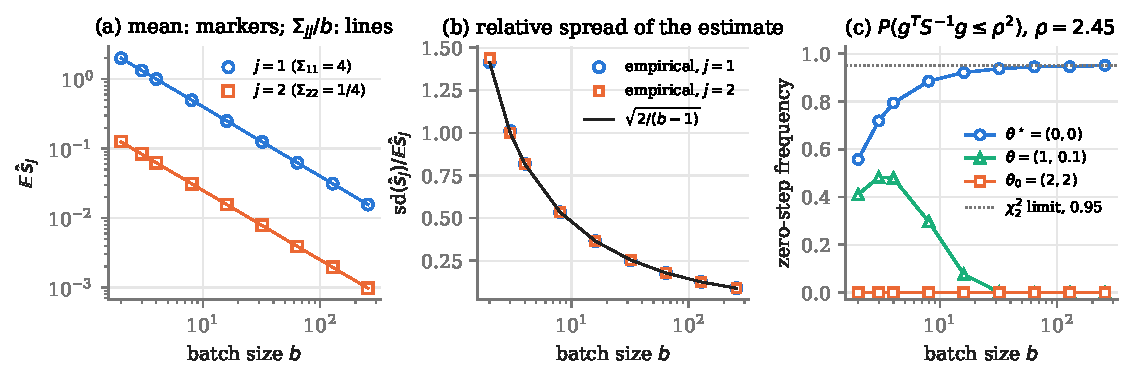
\includegraphics[width=\linewidth]{../fig/batch_size.pdf}
\caption{Размер батча и оценка неопределённости (квадратичная задача, $\sigma=1$,
$20\,000$ батчей на каждое $b$). (a) $\E\widehat s_j$ следует $\Sigma_{jj}/b$.
(b) Относительный разброс следует $\sqrt{2/(b-1)}$. (c) Доля нулевых шагов при
$\rho=2.45$ в трёх точках; в $\theta^\star$ она стремится к значению $0.95$ для
$\chi^2_2$.}
\label{fig:batch}
\end{figure}

Как читать результаты:
\begin{itemize}
\item Пункты 1 и 2 из 5.1 подтверждаются в пределах ошибки Монте-Карло при всех $b$
(отношения $1.00\pm0.013$; разброс отличается от $\sqrt{2/(b-1)}$ не более чем на
$0.025$).
\item Среднее $g^TS^{-1}g$ в $\theta^\star$ совпадает с $p(b-1)/(b-3)$ при $b\ge8$.
При $b=2,3$ теоретическое среднее бесконечно, и выборочные средние (788 и 13) ничего не
значат; при $b=4$ бесконечна дисперсия статистики, поэтому выборочное среднее сходится
медленно (5.3 против 6.0). Это эффект тяжёлых хвостов оценки дисперсии по двум-трём
точкам.
\item В $\theta_{\rm mid}$ доля нулевых шагов падает примерно с $0.4$--$0.5$ до $0$
между $b=4$ и $b=32$: переход происходит там, где $b\,\mu^T\Sigma^{-1}\mu\approx\rho^2$,
то есть при $b\approx6/0.89\approx7$. При $b\le4$ доля \emph{не} монотонна: при очень
маленьком батче $\widehat s_j$ часто случайно оказывается крошечной, $g^TS^{-1}g$
резко растёт, и нулевого шага не происходит. Поэтому решения о нулевом шаге при $b\le4$
в значительной степени случайны.
\item Робастная поправка убывает как $1/\sqrt b$: от $b=64$ к $b=256$ относительное
изменение уменьшается вдвое ($0.237\to0.117$). При фиксированном $\rho$ R-SGD с большим
$b$ почти совпадает с SGD.
\end{itemize}

\subsection*{5.3 Почему выбор с возвращением}

В обучаемых моделях наблюдения берутся из конечной обучающей выборки размера $n$. С
возвращением $b$ выборок независимы и одинаково распределены, и
$\E\widehat s_j=\Var(g_j)$ точно. Без возвращения дисперсия среднего по батчу получает
множитель конечной совокупности $(n-b)/(n-1)$, а выборочная дисперсия по-прежнему
оценивает дисперсию совокупности, поэтому $\widehat s_j$ завышает $\Var(g_j)$ в
$n/(n-b)$ раз. Проверка на данных логистической регрессии с $n=64$, $\sigma=0$,
$20\,000$ батчей:

\begin{center}
\begin{tabular}{@{}ccccc@{}}
\toprule
$n$ & $b$ & $\E\widehat s_j/\Var(g_j)$, с возвр. & без возвр. & прогноз $n/(n-b)$ \\
\midrule
64 & 8 & 1.000--1.002 & 1.139--1.143 & 1.143 \\
64 & 32 & 0.999--1.003 & 2.000--2.004 & 2.000 \\
\bottomrule
\end{tabular}
\end{center}
(Диапазоны — по трём координатам $w_1,w_2,c$.) Без возвращения при $b=n/2$
неопределённость была бы завышена вдвое, что приводило бы к ложным нулевым шагам.

\section*{Шаг 6. Пункт (d): что нужно для воспроизведения результатов}

\begin{itemize}
\item \textbf{Код.} \texttt{rsgd.py} (оценка (4), решатель, цикл SGD/R-SGD, оракулы,
генераторы данных, проверка конечными разностями) и \texttt{checks\_section2.py} (все
числа, таблицы и рисунки этого отчёта). Запуск: \texttt{python checks\_section2.py};
полный прогон занимает около 20\,с.
\item \textbf{Случайные числа.} Один главный сид $20261117$; эксперименты используют
независимые дочерние потоки \texttt{numpy.random.SeedSequence(20261117).spawn(8)}.
Внутри одного запуска оптимизации два отдельных генератора: для индексов батча и для
шума градиента $z_{k,i}$ (в разделе 3 ещё по одному для данных и для инициализации).
\item \textbf{Общие случайные числа.} SGD и R-SGD запускаются со свежими генераторами с
одинаковыми сидами, поэтому в парном сравнении они получают одни и те же индексы батчей и
одни и те же $z_{k,i}$ на каждой итерации (наблюдения всё же различаются, как только
расходятся итерации, поскольку $u_i$ вычисляется в разных $\theta_k$).
\item \textbf{Модель искажения.} Шум добавляется только к наблюдениям $V$. Целевая
функция $f$, обучающие данные, все потери и точности вычисляются на чистых данных.
\item \textbf{Настройки.} Везде float64; $b$, $\alpha_0$, расписание
$\alpha_0/\sqrt{1+k/50}$, число обновлений $K$, $\rho$, $\sigma$, $\theta_0$ — как указано
в каждой проверке; $\varepsilon_k$ строго по (4); допуски решателя $|\psi|\le10^{-14}$,
относительный шаг $\le10^{-15}$, не более 100 итераций; нулевой шаг фиксируется только
при $g^TS^{-1}g\le\rho^2$.
\item \textbf{Что сохраняется для каждого запуска.} Число вычислений градиента ($bK$ для
обоих методов), время, число нулевых шагов, итерации Ньютона, максимальная невязка 1(d).
\item \textbf{ПО.} Python 3.13.18, NumPy 2.5.3, SciPy 1.18.1, Matplotlib 3.11.2,
CVXPY 1.9.3 (Clarabel) — только для перекрёстной проверки.
\end{itemize}

\section*{Выводы для следующих разделов}

\begin{itemize}
\item Решатель точен с точностью до округления, надёжен и дёшев по числу операций; в
чистом Python его постоянные накладные расходы делают обновление R-SGD в 2--4 раза
медленнее обновления SGD для моделей с 3 и 33 параметрами, поэтому время нужно
указывать рядом с числом вычислений градиента.
\item Нулевой шаг — утверждение об отношении сигнал/шум градиента по мини-батчу, а не о
стационарности. Нулевые шаги появляются далеко от минимума, когда шум велик в
направлении малой кривизны.
\item $\rho$, $b$ и уровень шума взаимодействуют: область нулевого шага масштабируется как
$\rho\sigma/\sqrt b$, а робастная поправка — как $\rho/\sqrt b$. Честное сравнение в
разделе 4 должно настраивать $\rho$ при фактически используемом размере батча. Поскольку
поправка в значительной степени сводится к укорочению шага, её нужно сравнивать с SGD с
меньшим $\alpha_0$.
\item При $b\le4$ оценка $S_k$ слишком шумная (относительный разброс $\ge82\%$) для
надёжных решений о нулевом шаге; разумно брать $b\ge8$.
\end{itemize}

\textbf{Литература.}
J.~J.~Moré, D.~C.~Sorensen, Computing a trust region step, \emph{SIAM J.\ Sci.\
Stat.\ Comput.} 4 (1983) 553--572.
J.~Nocedal, S.~J.~Wright, \emph{Numerical Optimization}, 2nd ed., Springer, 2006, §4.3.

\section*{Приложение: решатель}

\begin{lstlisting}[language=Python]
def robust_step(g, s, alpha, rho, tol=1e-14, maxit=100):
    kappa2 = np.sum(g * g / s)                    # g^T S^{-1} g
    if rho == 0.0:                                # SGD
        return -alpha * g
    if kappa2 <= rho * rho:                       # zero-step rule (3)
        return np.zeros_like(g)
    a = alpha**2 * s * g * g                      # q(tau) = sum a/(tau+c)^2
    c = alpha * rho * s
    def psi_and_deriv(tau):
        den = tau + c
        q, dq = np.sum(a / den**2), -2.0 * np.sum(a / den**3)
        return q**-0.5 - 1.0, -0.5 * q**-1.5 * dq
    lo, hi = 0.0, alpha * np.sqrt(np.sum(s * g * g))   # bracket
    tau = 0.0
    psi, dpsi = psi_and_deriv(tau)
    for it in range(maxit):
        tau_new = tau - psi / dpsi                # Newton (monotone from 0)
        if not (lo < tau_new <= hi):
            tau_new = 0.5 * (lo + hi)             # safeguard, never used
        step, tau = abs(tau_new - tau), tau_new
        psi, dpsi = psi_and_deriv(tau)
        lo, hi = (tau, hi) if psi < 0 else (lo, tau)
        if abs(psi) <= tol or step <= 1e-15 * tau:
            break
    return -alpha * tau * g / (tau + c)
\end{lstlisting}

\end{document}
